% ============================ Enrico Ribiani 16-03-2021 ====================================================================
% Base per i documenti  
\documentclass[12pt]{article}
% ------------ pacchetti necessari ----------------
\usepackage[a4paper, total={6in, 8in},margin=1in]{geometry} % formattazione decente della pagina
\usepackage{graphicx}                            % need for figure
\usepackage{amsmath}
\usepackage{amsfonts}                            % if you want the fonts
\usepackage{amssymb}                             % if you want extra symbols
\usepackage{graphicx}  
\renewcommand{\figurename}{Figura}  
\renewcommand{\contentsname}{Indice}                        % need for figures
\usepackage{mathptmx}
\usepackage{float}                               % serve per mettere tabelle e immagini dove si vuole 
\usepackage[utf8]{inputenc}
\usepackage{textcomp}
\usepackage[hang,flushmargin,bottom]{footmisc}   % footnote format
\usepackage{fancyhdr, lastpage}
\usepackage{titlesec}
\usepackage[table,dvipsnames]{xcolor}
%\pagestyle{fancy}
%\renewcommand{\headrulewidth}{0pt}
%\renewcommand*\contentsname{Indice}
\titleformat{\section}{\normalsize\bfseries}{\thesection.}{1em}{}	% required for heading numbering style
\titleformat*{\section}{\Large\bfseries}
\titleformat*{\subsection}{\large\bfseries}
%\usepackage{siunitx}
%\usepackage{tikz}
\usepackage{circuitikz}
%\usepackage[siunitx]{circuitikz}
\usepackage{multirow}
%===================links=================
\usepackage{hyperref}
\hypersetup{
    colorlinks=true,
    linkcolor=Sepia,
    filecolor=Green,      
    urlcolor=Cyan,
    pdftitle={SAMPLE},
    pdfpagemode=FullScreen,
    }
%===================inizio pagina del titolo=================
\begin{document}
    \begin{titlepage}
    \begin{center}
% ------------------ inizio immagine logo ----------
\begin{figure}
    \centering
    
\includegraphics{~/varie/logo.png}
    \label{fig:logo}
\end{figure}
% ------------------ fine immagine logo ----------
% ------------------ fine immagine logo ----------
-------------------------------------------------------------------------------------\\
\vspace{2\baselineskip}
\large Enrico Ribiani\\
\large 3AUB\\
\vfill

\Huge{\textbf{Esperienza laboratoriale bipolo ohmico-capacitivo}}\\
\vfill

\LARGE{esperienza n°1}\\
\vfill
\large{01-10-2021}
\end{center}
%=============== fine pagina titolo ===============
\end{titlepage}
\tableofcontents
\vskip 1cm
\section{Scopo:Verificare il comportamento di un bipolo ohmico-capacitivo sperimentalmente.}
    \subsection{Materiale}
    \begin{itemize}
        \item Breadboard
        \item Condensatore da \textit{10nF}
        \item Resistenza da \textit{10k$\Omega$}
        \item Breadboard
    \end{itemize}
    \subsection{Strumenti}
    \begin{itemize}
        \item Generatore di funzione
        \item Oscilloscopio
    \end{itemize}
        \subsubsection{Schema}
        \begin{circuitikz}[american voltages]
            \draw
                (0,0) -- (0,-0.2) node[ground]{}    
                to[vsourcesin, l_=\textit{v(t)}] (0,4)
                (0,4) to [short, *-, l=Ch1] (0,4)
                to[american resistor,  l_=R \textit{10k$\Omega$}, i=\textit{i(t)}] (4,4) -- (4,0)
                (4,4) to [short, *-, l=Ch2] (4,0) %label ch2 da fixare
                to[capacitor, l=C\textit{10nF}] (0,0)
                (0,0) to [short, *-] (0,0)
            ;
        \end{circuitikz}

        \vskip 1cm
        
        \begin{center}
            Il primo circuito verrà utilizzato per effettuare le misure su R mentre il secondo che è l'equivalente del primo solo con R e C invertiti
            per effettuare le misurazioni su C.\\
        \end{center}
       
        \vskip 1cm

   \begin{circuitikz}[american voltages]
    \draw
        (0,0) -- (0,-0.2) node[ground]{}    
        to[vsourcesin, l_=\textit{v(t)}] (0,4)
        (0,4) to [short, *-, l=Ch1] (0,4)
        to[capacitor, l=C \textit{10nF}] (4,4) -- (4,0)
        (4,4) to [short, *-, l_=Ch2,i=\textit{i(t)}] (4,0) %label ch2 da fixare
        to[american resistor,  l_=R \textit{10k$\Omega$}] (0,0)
        (0,0) to [short, *-] (0,0)
    ;
\end{circuitikz}

\section{Cenni teorici}
    \subsection{Generalità bipolo RC} 
    \subsection{Previsione comportamento}
\section{Procedimento/Analisi}
    \subsection{Tabelle}
    \begin{center}
        \begin{tabular}{|p{2cm}|p{2cm}|p{2cm}|} 
        \hline
        \rowcolor{BurntOrange} \multicolumn{3}{|c|}{C} \\
        \hline\hline
        \rowcolor{Apricot} Vpp & t$\pm$ & $\varphi$  \\ 
         \hline
        \rowcolor{Peach}6V & -90$\mu$s & -32,4°  \\
         
         \hline
        \end{tabular}
        \vspace{1cm}
            \begin{tabular}{|p{2cm}|p{2cm}|p{2cm}|} 
            \hline
            \rowcolor{BurntOrange} \multicolumn{3}{|c|}{R} \\
            \hline\hline
            \rowcolor{Apricot} Vpp & t$\pm$ & $\varphi$  \\ 
             \hline
            \rowcolor{Peach}3,56V & 170$\mu$s & 61,2°  \\
             
             \hline
            \end{tabular}
\end{center}
    \subsection{Calcoli}
    Incognite: $\vec{Z}$, $\vec{V}$, $\vec{V_R}$, $\vec{V_C}$, $\vec{I}$\\
    \\
    $Vp=\frac{Vpp}{2}=\frac{7V}{2}=3,5V$\\
    $V=\frac{Vp}{\sqrt{2}}=\frac{3,50V}{\sqrt{2}}=2,47V$\\
    \\
    $Vp_R=\frac{Vpp_R}{2}=\frac{3,56V}{2}=1,78V$\\
    $V_R=\frac{Vp_R}{\sqrt{2}}=\frac{1,78V}{\sqrt{2}}=1,26V$\\
    \\
    $Vp_C=\frac{Vpp_C}{2}=\frac{6V}{2}=3V$\\
    $V_C=\frac{Vp_C}{\sqrt{2}}=\frac{3V}{\sqrt{2}}=2,12V$\\
    \\
    $X_c=\frac{1}{\omega C}=\frac{1}{2\pi f C}=\frac{1}{2\pi\cdot 1000 \cdot 10^{-9}}=159,15k\Omega$\\
    \\
    $\varphi:2\pi=-90\cdot 10^{-6}:0,001$ \\
    $\varphi=\frac{2\pi \cdot (-90\cdot 10^{-6})}{0,001}=-32,4$°\\
    \\
    \\
    $\vec{Z}=(R-jX_C)=(10-159,15)k\Omega$\\
    $Z=\sqrt{10000^2+159150^2}=159,5k\Omega$\\
    \\
    $I=\frac{V}{Z}=\frac{2,47V}{159500\Omega}=15\mu A$\\
\section{Conclusioni}
\subsection{Diagramma vettoriale}
\begin{figure}[H]
    \centering
    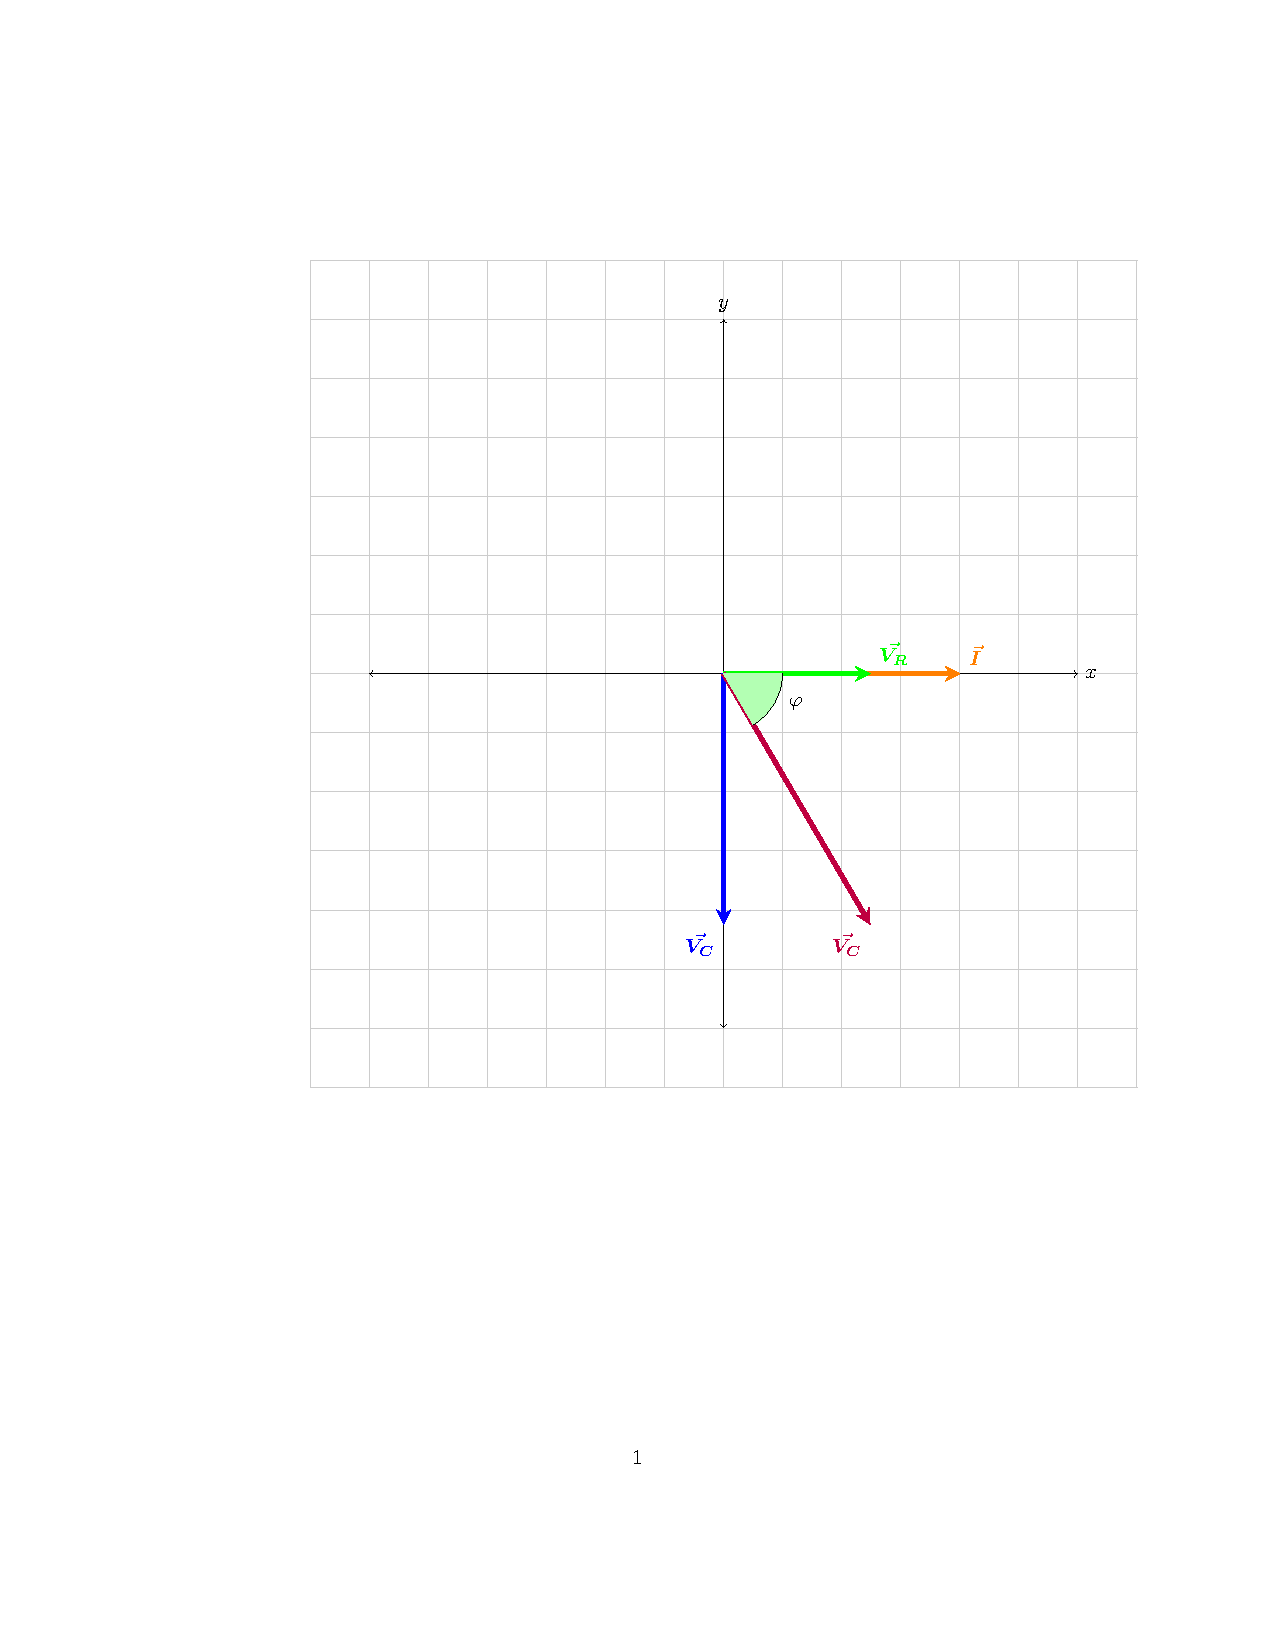
\includegraphics[scale=0.7]{diagramma-vettoriale.pdf}
\end{figure}
\end{document}
